\documentclass[10pt, a4paper]{article}
\usepackage[top=0.6in,bottom=1.0in,left=1.0in,right=1.0in]{geometry}
\usepackage{amsmath,amssymb}
\usepackage{hyperref}
\fontfamily{times}
\usepackage{graphicx,float,tikz}

\title{ \large CS 4366: Senior Capstone Project \\ Dr. Sunho Lim \\ Project \#1 - Project Plan - Project Report \\ EmergenSeek}
\author{Suhas Bacchu \ Derek Fritz \ Kevon Manahan \ Annie Vo \ Simon Woldemichael}
\date{January 30, 2019}

\begin{document}

\maketitle
\vspace{-1cm}
\begin{abstract}
In this report, we propose the development of a mobile application which will provide users with multiuse, centralized emergency information and notification. This application will provide friends and family members with priority connections in times of emergency or crisis.
\end{abstract}

\section{Problem Definition and Motivation}
\par ~ Many people look to travel as a means of discovering new experiences and enjoying brief respites in the middle of their busy lives. Outside of leisure, many companies encourage their employees to travel frequently in the form of consulting roles and teams spread across multiple branches. Many universities, likewise, are promoting studying abroad in order for their students to gain a broader view of the world. In 2017, a total of 2.25 billion person-trips were made domestically and another 76.9 million internationally \cite{one}. The sheer quantity of people traveling is enormous, and the number continues to grow every passing year as more options are made available.

\par ~ Road travel makes up a large portion of these trips. The United States is one of the busiest countries in terms of road traffic with nearly 264 million vehicles registered and 218 million drivers holding a valid driving license \cite{two}. That accounts for almost 70\% of the population of the United States  \cite{two}. The level of traffic is one of the reasons leading to more traffic accidents. Road trips represented some 22 percent of vacations taken by United States travelers in 2015, jumping to 39 percent the following year, according to MMGY Global’s 2017-18 Portrait of American Travelers. Seeking convenience and adventure (while avoiding airport security, baggage fees, and the hassle of flying with young children or pets), more travelers are hitting the road to explore unfamiliar places.

\par ~ With these growing numbers, however, the strictness of regulations continues to impose greater restrictions on travelers. The logistics of planning a trip grow more complex by the day, and this can result in a large amount of stress for potential travelers. Additionally, many people possess concerns regarding safety while traveling to unfamiliar destinations. Daily news stories about violence in large cities and health concerns in developing countries have instilled a general apprehension towards travel.

\par ~ It is highly evident that the stress of travel compounded with these very real concerns may discourage many individuals from experiencing the joys of travel. The worry of safety and well-being should not be a factor which should discourage travel, in the highly technologically advanced world that we live in today.

\section{System Overview}
\par ~ Herein lies our motivation for proposing an all-in-one, travel-friendly emergency service locator. EmergenSeek aims to alleviate some of the worries that travelers may possess, providing peace-of-mind for travelers and their families regardless of where they may be. By keeping selected family and friends updated on the traveler’s location and safety, informing the user of nearby health service options, and allowing for instantaneous assistance in the form of an SOS button, we hope that EmergenSeek will instill people with a sense of safety, even in unfamiliar locations.

\par ~ While serving primarily as a platform for traveler safety, EmergenSeek possesses countless other applications as well. For instance, if a burglar breaks into your house, your neighbor keels over in her yard or you witness a major car crash, one’s default assumption would be to dial 911. “Where is your emergency?” is the first question dispatchers ask because a location is the top piece of information they need to send help. According to the Federal Communications Commission, the dispatcher might not be able to pinpoint exactly where you’re calling from if you’re calling from your cellphone. Additionally, you might lack the composure to convey key information to the dispatcher when placed in an urgent situation. With EmergenSeek’s accessibility and instantaneous emergency features, users may notify all of their selected contacts with their current location.

\par ~ EmergenSeek, at its core, is a location-based service (LBS), providing key information to the user based on their location and proximity to useful services. The platform is designed to be implemented as a mobile application, fulfilling the core need of instant and accessible assistance in urgent situations. Around this mobile application are the managed systems and infrastructure provided by Amazon Web Services, logically connected using the Go programming language, Twilio’s Programmable Voice and SMS APIs, and Google’s Maps and Geocoding APIs.

The following features have been selected as central to our system, and may be expanded upon through development:
\begin{enumerate}
\item[1.] Location-based notification of health services (pharmacies, hospitals, etc.) 
\item[2.] A customizable contacts list that allows for varying levels of information sharing. Example: Family members will have full and priority access on the location metadata of an application user, but friends and acquaintances will have filtered permissions on viewing information about the application user. This granular permissions system will allow for full control of privacy by the user.
\item[3.] Real-time polling of location data, which will be sent to specified contacts and tracked via other instances of the application for assisting in moments of emergency (i.e. SOS mode).
\item[4.] An emergency situation SOS button, which will broadcast an alert to specified contacts and display emergency information in an accessible format (e.g. on the lock screen for first responders to view if the application user becomes unresponsive).
	\begin{itemize}
		\item[a.] Additionally, using this button and leveraging Twilio’s Programmable Voice and SMS API, we will contact the application user’s pre-defined primary contacts and family members in an automated fashion.
	\end{itemize}
\item[5.] User profile options and personalization, including sign-in functionality via a third party OAuth provider such as Google and Facebook so that users may sync their EmergenSeek account information with their already active social media accounts.
\end{enumerate}

\section{Expected Outcomes and Improvements}
\par ~ From the development and progress of EmergenSeek, we as developers will have a better grasp of mobile application development through Android, API development using the Go programming language and AWS DocumentDB for data persistence, and a working understanding of leveraging Amazon Web Services’ various offerings to successfully produce and deploy.

\par ~ With the public release of the app, we hope for end-users from all demographics and ages to have a go-to product which will alleviate their concerns in times of emergency as well as to calm the minds of worried family members who may have children, elderly, or other loved ones that may bring them concerns. The overall piece of mind that will be granted to the user of our application, and the user's loved ones, will make traveling, anywhere in the world, even more of an enjoyable experience.

\par ~ Additionally, we also hope that the application will aid users in developing good habits in times of distress. In urgent situations, panic and anxiety may prevent those in need from thinking clearly. With the utility of our application, however, this panic and anxiety will be reduced down to routine actions which will ensure for optimal safety and security.

	\begin{figure}[H]
	\begin{center}	
	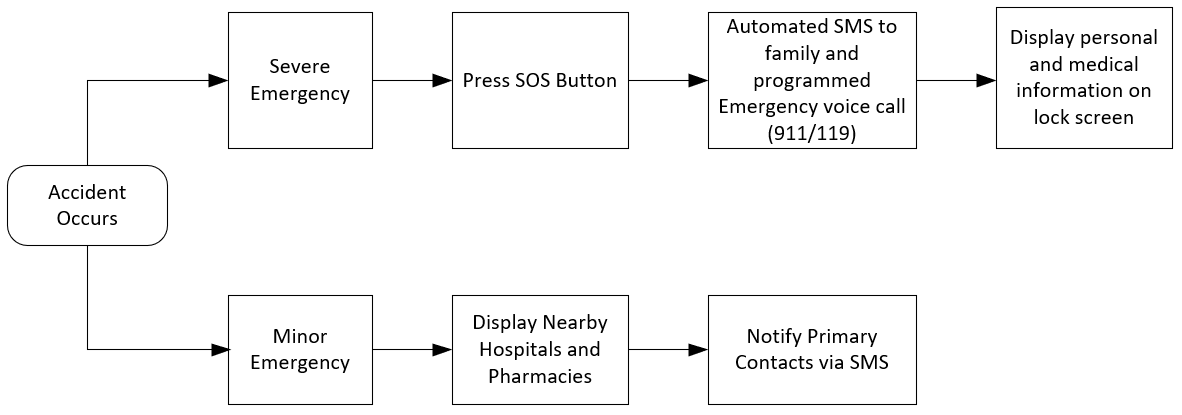
\includegraphics[scale=.40]{accident-flowchart.PNG}
	\caption{A flowchart showing the logical steps which take place in two different severity levels of accident occurrence.}
	\label{fig:1}	
	\end{center}	
	\end{figure}
	
\par ~ For instance, take the diagram above which outlines a single use-case when the application user has gotten into an accident (car or otherwise). If the accident is serious, the user simply needs to open the application, hit the SOS button, and have the piece of mind of knowing that their distress single has been sent to the proper emergency services and their loved ones have been notified. If the accident is not of a large magnitude, then the application user will be able to quickly find nearby hospitals and pharmacies and have their current location sent to only primary contacts (spouse, guardian, parents, children, siblings, etc.).
	
\begin{thebibliography}{9}
\bibitem{one}
U.S. TRAVEL AND TOURISM OVERVIEW (2017): \url{https://www.ustravel.org/system/files/media_root/document/Research_Fact-Sheet_US-Travel-and-Tourism-Overview.pdf}
\bibitem{two}
Number of licensed drivers in the United States from 1990 to 2016 (in 1,000s): \url{https://www.statista.com/statistics/191653/number-of-licensed-drivers-in-the-us-since-1988/}
\end{thebibliography}
\end{document}

